\documentclass[border=6pt]{standalone}
\usepackage{fontspec}
\usepackage{xeCJK}
\usepackage{xcolor}
\usepackage{tikz}
\usetikzlibrary{
    arrows.meta,
    backgrounds,
    calc,
    decorations.pathreplacing,
    fit,
    positioning,
    shapes.geometric
}

\setmainfont{Times New Roman}
\setsansfont{Noto Sans SC}
\setCJKmainfont{Noto Sans SC}
\setCJKsansfont{Noto Sans SC}

\definecolor{ink}{HTML}{1F2937}
\definecolor{muted}{HTML}{64748B}
\definecolor{lineblue}{HTML}{2563EB}
\definecolor{prefill}{HTML}{E7F0FF}
\definecolor{prefillLine}{HTML}{2F5597}
\definecolor{decode}{HTML}{EAF7EA}
\definecolor{decodeLine}{HTML}{2F7D32}
\definecolor{kv}{HTML}{FFF3D8}
\definecolor{kvLine}{HTML}{B7791F}
\definecolor{accent}{HTML}{FDE8E8}
\definecolor{accentLine}{HTML}{C2410C}
\definecolor{panel}{HTML}{F8FAFC}
\definecolor{panelLine}{HTML}{94A3B8}
\definecolor{violet}{HTML}{F1ECFF}
\definecolor{violetLine}{HTML}{6D28D9}
\definecolor{teal}{HTML}{DFF7F3}
\definecolor{tealLine}{HTML}{0F766E}

\tikzset{
    every picture/.style={font=\sffamily},
    title/.style={font=\sffamily\bfseries\Large, text=ink},
    subtitle/.style={font=\sffamily\small, text=muted, align=center},
    block/.style={
        draw=panelLine,
        rounded corners=5pt,
        fill=white,
        line width=0.8pt,
        align=center,
        inner xsep=7pt,
        inner ysep=6pt
    },
    pblock/.style={block, fill=prefill, draw=prefillLine},
    dblock/.style={block, fill=decode, draw=decodeLine},
    kvblock/.style={block, fill=kv, draw=kvLine},
    warnblock/.style={block, fill=accent, draw=accentLine},
    vblock/.style={block, fill=violet, draw=violetLine},
    tblock/.style={block, fill=teal, draw=tealLine},
    cluster/.style={
        draw=panelLine,
        rounded corners=6pt,
        fill=panel,
        line width=0.8pt,
        inner sep=8pt
    },
    arrow/.style={-{Latex[length=3mm,width=2mm]}, draw=ink, line width=0.85pt},
    bluearrow/.style={arrow, draw=prefillLine},
    greenarrow/.style={arrow, draw=decodeLine},
    kvarrow/.style={arrow, draw=kvLine},
    orangearrow/.style={arrow, draw=accentLine},
    control/.style={-{Latex[length=2.6mm,width=1.8mm]}, draw=muted, line width=0.75pt, dashed},
    label/.style={font=\sffamily\scriptsize, text=muted, align=center},
    small/.style={font=\sffamily\scriptsize, align=center},
    rank/.style={
        draw=panelLine,
        rounded corners=3pt,
        fill=white,
        minimum width=12mm,
        minimum height=6mm,
        font=\sffamily\scriptsize,
        align=center
    },
    head/.style={
        draw=ink,
        line width=0.35pt,
        minimum width=6.5mm,
        minimum height=4.8mm,
        font=\sffamily\tiny,
        align=center
    },
    metric/.style={
        draw=panelLine,
        rounded corners=4pt,
        fill=white,
        font=\sffamily\scriptsize,
        align=center,
        inner xsep=5pt,
        inner ysep=4pt
    }
}


\begin{document}
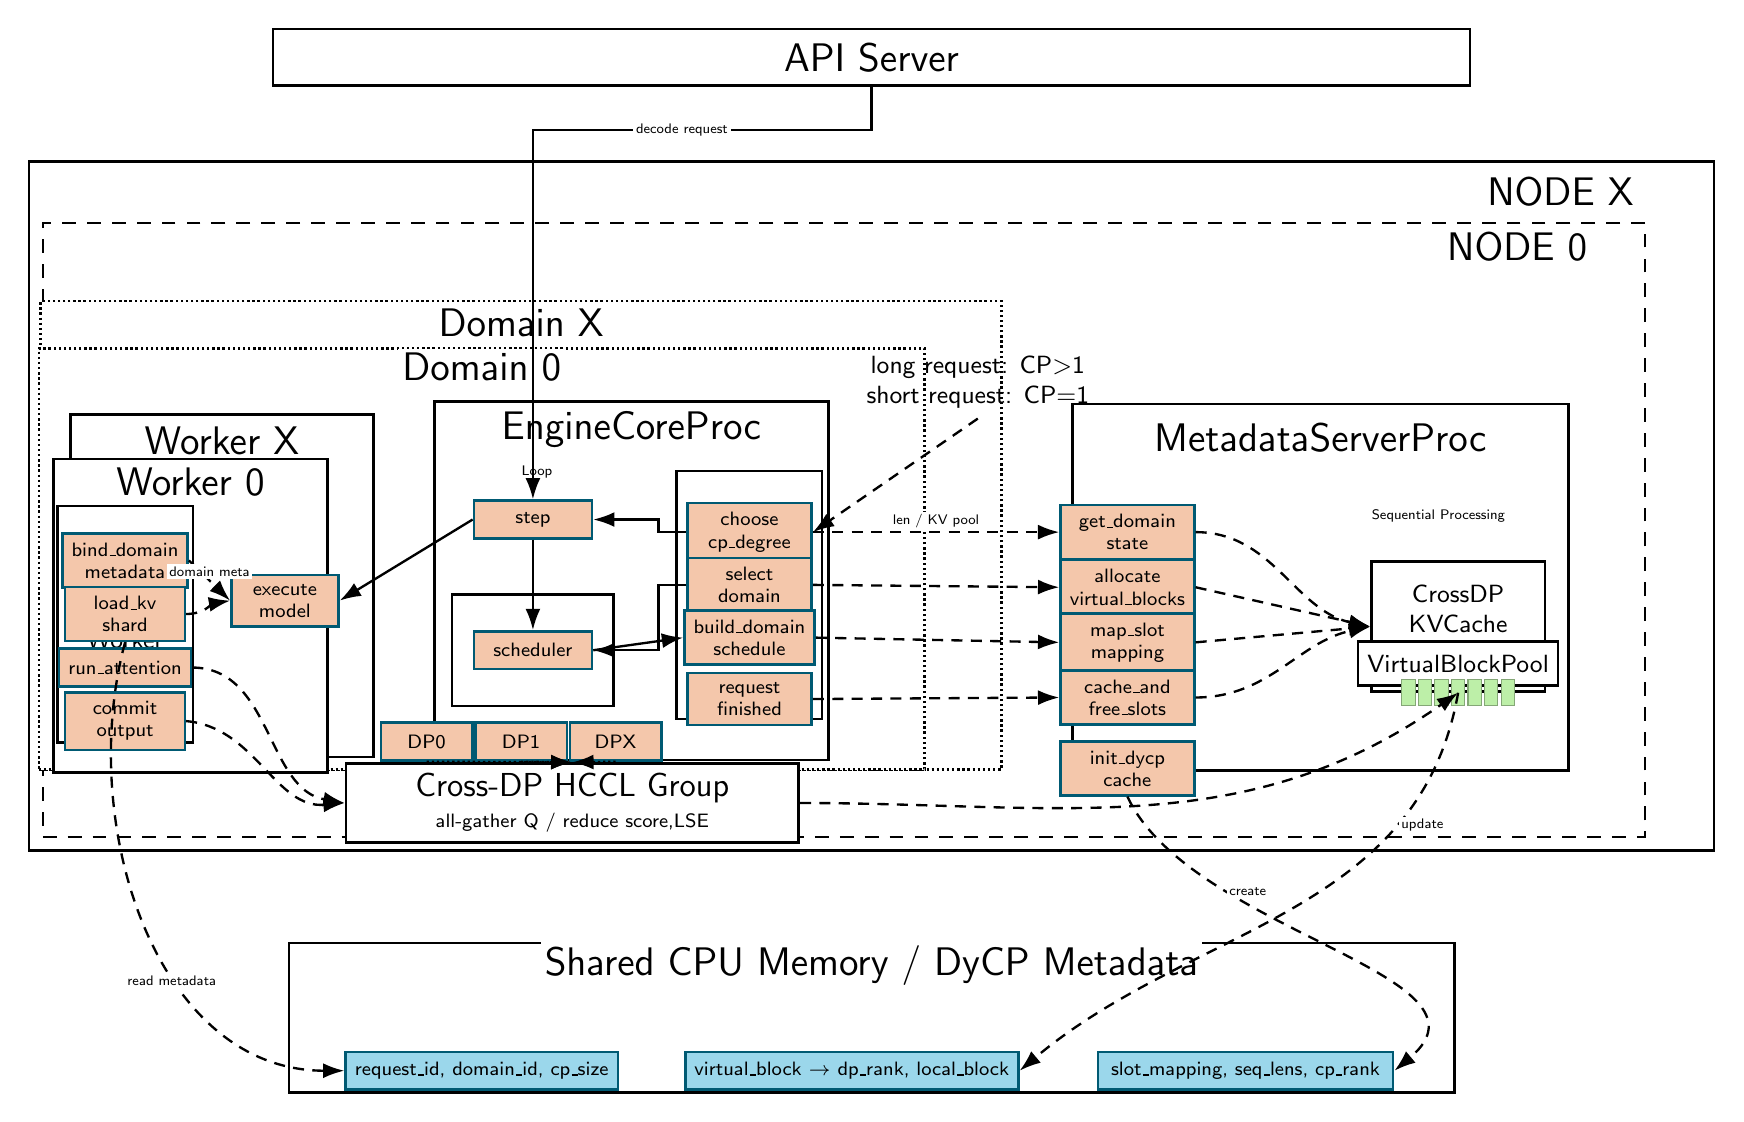
\begin{tikzpicture}[x=1cm,y=1cm]
    \definecolor{dyPeach}{HTML}{F4C7AB}
    \definecolor{dyBlue}{HTML}{005A73}
    \definecolor{dyMem}{HTML}{9BD7EB}
    \definecolor{dyGreen}{HTML}{BDEFA8}

    \tikzset{
        frame/.style={draw=black, fill=white, line width=0.85pt},
        outerframe/.style={frame, line width=0.95pt, align=center},
        dashframe/.style={frame, dashed, dash pattern=on 5pt off 4pt},
        dotframe/.style={frame, densely dotted, line width=0.95pt},
        proc/.style={frame, align=center, font=\sffamily\large},
        smallproc/.style={frame, align=center, font=\sffamily\small},
        method/.style={
            draw=dyBlue,
            fill=dyPeach,
            line width=0.9pt,
            align=center,
            font=\sffamily\scriptsize,
            minimum height=0.48cm
        },
        memory/.style={
            draw=dyBlue,
            fill=dyMem,
            line width=0.9pt,
            align=center,
            font=\sffamily\scriptsize,
            minimum height=0.48cm
        },
        pool/.style={
            draw=black,
            fill=white,
            line width=0.85pt,
            align=center,
            font=\sffamily\small
        },
        dataarrow/.style={-{Latex[length=2.7mm,width=1.9mm]}, draw=black, line width=0.85pt},
        metaarrow/.style={-{Latex[length=2.7mm,width=1.9mm]}, draw=black, line width=0.85pt, dashed, dash pattern=on 4pt off 3pt},
        commarrow/.style={-{Latex[length=2.7mm,width=1.9mm]}, draw=black, line width=0.85pt, densely dotted},
        tinylabel/.style={font=\sffamily\tiny, align=center, fill=white, inner sep=1pt}
    }

    \node[outerframe, minimum width=15.2cm, minimum height=0.72cm, font=\sffamily\Large] (api) at (11.0,13.25) {API Server};

    \node[outerframe, minimum width=21.4cm, minimum height=8.75cm] (nodex) at (11.0,7.55) {};
    \node[font=\sffamily\Large] at (19.75,11.55) {NODE X};
    \node[dashframe, minimum width=20.35cm, minimum height=7.8cm] (node0) at (10.65,7.25) {};
    \node[font=\sffamily\Large] at (19.2,10.85) {NODE 0};

    \node[dotframe, minimum width=12.2cm, minimum height=5.95cm] (domainx) at (6.55,7.18) {};
    \node[font=\sffamily\Large, fill=white, inner sep=1.5pt] at (6.55,9.88) {Domain X};
    \node[dotframe, minimum width=11.25cm, minimum height=5.35cm] (domain0) at (6.05,6.88) {};
    \node[font=\sffamily\Large, fill=white, inner sep=1.5pt] at (6.05,9.32) {Domain 0};

    \node[outerframe, minimum width=3.85cm, minimum height=4.35cm] (workerx) at (2.75,6.54) {};
    \node[font=\sffamily\Large] at (2.75,8.38) {Worker X};
    \node[outerframe, minimum width=3.48cm, minimum height=3.98cm] (worker0) at (2.35,6.16) {};
    \node[font=\sffamily\Large] at (2.35,7.86) {Worker 0};
    \node[pool, minimum width=1.72cm, minimum height=3.0cm] (dyworker) at (1.52,6.05) {DyCP\\Worker};
    \node[method, minimum width=1.52cm] (w-bind) at (1.52,6.86) {bind\_domain\\metadata};
    \node[method, minimum width=1.52cm] (w-load) at (1.52,6.18) {load\_kv\\shard};
    \node[method, minimum width=1.52cm] (w-attn) at (1.52,5.5) {run\_attention};
    \node[method, minimum width=1.52cm] (w-commit) at (1.52,4.82) {commit\\output};
    \node[method, minimum width=1.36cm] (execute) at (3.55,6.35) {execute\\model};

    \node[outerframe, minimum width=5.0cm, minimum height=4.55cm] (engine) at (7.95,6.6) {};
    \node[font=\sffamily\Large] at (7.95,8.52) {EngineCoreProc};
    \node[font=\sffamily\tiny] at (6.75,7.98) {Loop};
    \node[method, minimum width=1.5cm] (step) at (6.7,7.38) {step};
    \node[pool, minimum width=2.05cm, minimum height=1.42cm] (schedbox) at (6.7,5.72) {};
    \node[method, minimum width=1.5cm] (scheduler) at (6.7,5.72) {scheduler};
    \node[pool, minimum width=1.85cm, minimum height=3.15cm] (cdps) at (9.45,6.42) {CrossDP\\Scheduler};
    \node[method, minimum width=1.58cm] (choose) at (9.45,7.22) {choose\\cp\_degree};
    \node[method, minimum width=1.58cm] (select) at (9.45,6.55) {select\\domain};
    \node[method, minimum width=1.58cm] (build) at (9.45,5.88) {build\_domain\\schedule};
    \node[method, minimum width=1.58cm] (finished) at (9.45,5.1) {request\\finished};

    \node[outerframe, minimum width=6.3cm, minimum height=4.65cm] (meta) at (16.7,6.52) {};
    \node[font=\sffamily\Large] at (16.7,8.42) {MetadataServerProc};
    \node[method, minimum width=1.7cm] (m-state) at (14.25,7.22) {get\_domain\\state};
    \node[method, minimum width=1.7cm] (m-alloc) at (14.25,6.52) {allocate\\virtual\_blocks};
    \node[method, minimum width=1.7cm] (m-map) at (14.25,5.82) {map\_slot\\mapping};
    \node[method, minimum width=1.7cm] (m-free) at (14.25,5.12) {cache\_and\\free\_slots};
    \node[method, minimum width=1.7cm] (m-init) at (14.25,4.22) {init\_dycp\\cache};

    \node[pool, minimum width=2.2cm, minimum height=1.65cm, fill=white] (manager) at (18.45,6.02) {CrossDP\\KVCache\\Manager};
    \node[smallproc, minimum width=1.78cm, minimum height=0.56cm] (vpool) at (18.45,5.55) {VirtualBlockPool};
    \foreach \i/\x in {0/17.82,1/18.03,2/18.24,3/18.45,4/18.66,5/18.87,6/19.08} {
        \node[draw=dyGreen!70!black, fill=dyGreen, minimum width=0.17cm, minimum height=0.33cm, inner sep=0pt] at (\x,5.18) {};
    }
    \node[font=\sffamily\tiny] at (18.2,7.42) {Sequential Processing};

    \node[outerframe, minimum width=5.75cm, minimum height=1.0cm, font=\sffamily] (comm) at (7.2,3.78) {\large Cross-DP HCCL Group\\[-1pt]{\scriptsize all-gather Q / reduce score,LSE}};
    \node[method, minimum width=1.16cm] (dp0) at (5.35,4.56) {DP0};
    \node[method, minimum width=1.16cm] (dp1) at (6.55,4.56) {DP1};
    \node[method, minimum width=1.16cm] (dpx) at (7.75,4.56) {DPX};
    \node[font=\sffamily\small, align=center] (policy) at (12.35,9.12) {long request: CP$>$1\\short request: CP=1};

    \node[outerframe, minimum width=14.8cm, minimum height=1.9cm] (shared) at (11.0,1.05) {};
    \node[font=\sffamily\Large, fill=white, inner sep=1.5pt] at (11.0,1.72) {Shared CPU Memory / DyCP Metadata};
    \node[memory, minimum width=3.25cm] (mem1) at (6.05,0.38) {request\_id, domain\_id, cp\_size};
    \node[memory, minimum width=3.85cm] (mem2) at (10.75,0.38) {virtual\_block $\rightarrow$ dp\_rank, local\_block};
    \node[memory, minimum width=3.75cm] (mem3) at (15.75,0.38) {slot\_mapping, seq\_lens, cp\_rank};

    \draw[dataarrow] (api.south) -- ++(0,-0.55) -| node[tinylabel, pos=0.28] {decode request} (step.north);
    \draw[dataarrow] (step.west) -- (execute.east);
    \draw[dataarrow] (step.south) -- (scheduler.north);
    \draw[dataarrow] (scheduler.east) -- (build.west);
    \draw[dataarrow] (choose.west) -- ++(-0.35,0) |- (step.east);
    \draw[dataarrow] (select.west) -- ++(-0.35,0) |- (scheduler.east);

    \draw[metaarrow] (policy.south) -- (choose.east);
    \draw[metaarrow] (choose.east) -- node[tinylabel, above] {len / KV pool} (m-state.west);
    \draw[metaarrow] (select.east) -- (m-alloc.west);
    \draw[metaarrow] (build.east) -- (m-map.west);
    \draw[metaarrow] (finished.east) -- (m-free.west);
    \draw[metaarrow] (m-state.east) to[out=0,in=168] (manager.west);
    \draw[metaarrow] (m-alloc.east) -- (manager.west);
    \draw[metaarrow] (m-map.east) -- (manager.west);
    \draw[metaarrow] (m-free.east) to[out=0,in=192] (manager.west);

    \draw[metaarrow] (w-bind.east) -- node[tinylabel, above] {domain meta} (execute.west);
    \draw[metaarrow] (w-load.east) to[out=0,in=190] (execute.west);
    \draw[metaarrow] (w-attn.east) to[out=0,in=170] (comm.west);
    \draw[metaarrow] (w-commit.east) to[out=-5,in=185] (comm.west);

    \draw[commarrow] (dp0.south) -- (comm.north);
    \draw[commarrow] (dp1.south) -- (comm.north);
    \draw[commarrow] (dpx.south) -- (comm.north);
    \draw[metaarrow] (comm.east) to[out=0,in=-145] (manager.south);

    \draw[metaarrow] (w-load.south) to[out=-105,in=180] node[tinylabel, pos=0.6, below] {read metadata} (mem1.west);
    \draw[metaarrow] (m-init.south) to[out=-65,in=40] node[tinylabel, pos=0.28, right] {create} (mem3.east);
    \draw[metaarrow] (manager.south) to[out=-100,in=40] node[tinylabel, pos=0.25, right] {update} (mem2.east);
\end{tikzpicture}
\end{document}
